\chapter{Implementation}
\label{implementation}

In the~field of \zk{GIS}, users are dealing with a~huge amount of satellite photos.
Though there are many algorithms for automated classification, \zk{ANN}s are
a~promising child which is just growing up and hogging the~limelight. However,
the~younger sibling of \zk{ANN}s is even more promising. The~sibling is called 
\zk{CNN}s.

\zk{CNN}s for image processing are very strong in an object detection.
The~object detection in aerial photos could be very useful for example for detecting 
sick trees in an orthophoto of a~forest or for a~vehicle detection (aeroplane, 
ship, car, etc.). It means elements that can be represented as points. But what 
about searching for forests? Searching for lakes? Rivers? Oil spills? Do we 
really want to represent them in \zk{GIS} as points in their centre of mass?

It seems that better representation is in polygons (or lines). But representing
a detection bounding box as a~polygon square does not seem like the~right way. 
So there are two possible ways - semantic segmentation and instance 
segmentation. Three arguments were raised and discussed on behalf of instance 
segmentation:
\begin{itemize}
	\item The~instance differentiation could be very useful for some tasks.
	\item It is easier to create masks only for requested objects.
	\item If each pixel in a~raster input will be assigned to a~class, we got
	\textit{semantic segmentation}.
\end{itemize}

When works on this implementation started, the~paper on Mask R-CNN was just 
recently published (\cite{mask-rcnn}, March 2017). With its approach, it was
a~kind of bleeding edge. However, its results spoke for themselves and within
a~year of its publication, it was implemented in few projects following
the~success of the~original paper. Few followers also appeared (for example 
\cite{masklab}) and it could be interesting to examine them deeper from
a~geomatic point of view.

For the~implementation to GRASS GIS, the~Python language was chosen. There are
few reasons for this decision:
\begin{itemize}
	\item Although some GRASS GIS modules are written in C and C++, many of them
	are written in Python.
	\item Python allows me to use libraries such as TensorFlow and Keras, both
	very useful and widely used in the~field of deep learning. 
\end{itemize}

Mask \zk{R-CNN} tools created for the~practical part of the~thesis consist of 
two modules. \verb|ann.maskrcnn.train| allows the user to train a~Mask R-CNN model 
on his own dataset, \verb|ann.maskrcnn.detect| allows him to use that model to 
detect features in georeferenced files. Both modules are licensed under GNU
\zk{GPL}~2 license.

Along with these modules, a~library of Mask \zk{R-CNN} tools was prepared. This 
library was heavily based on a~Python implementation of Mask \zk{R-CNN} written 
by Waleed Abdulla from Matterport, 
Inc.\footnote{\url{https://matterport.com/about/}}  Matterport, Inc. published 
their implementation under the~MIT License \cite{mit}. The~MIT License is
a~license granting the~permission to use the~code, copy it, modify it, publish and 
even to sell it free of charge and is compatible with GNU \zk{GPL} 
2 (or newer) \cite{gplv2} of GRASS GIS. Scripts in the~library are also under 
the MIT License and moreover, Waleed Abdulla himself agreed with the~usage and 
modifications of his code for purposes of the~GRASS GIS usage. The~Matterport, 
Inc. Mask \zk{R-CNN} implementation can be found in their GitHub 
repository\footnote{\url{https://github.com/matterport/Mask\_RCNN}}.

The Matterport implementation of Mask \zk{R-CNN} was chosen because of many 
reasons. Besides its license compatibility, it is quite robust and ready for 
modifications leading to another implementation, so it saved thousands of lines 
of code. But the~main motivation behind its usage is that there is a~plenty of 
people interested in this project, proposing their ideas and testing it. And 
these people are experienced in fields of computer vision and deep learning, so 
besides the~base of GRASS \zk{GIS} users, there are always people from another 
field working with core functions of the~model. Even Abdulla himself is very 
active in answering people's questions and open-minded when discussing other 
people improvement proposals. I found it very useful and consider it as
the~icing on the~cake of open source software.

The following text will briefly describe the~structure of the~mentioned modules 
together with their workflow. Because aspects of the~Mask \zk{R-CNN} 
architecture were already mentioned in chapter \ref{mask-rcnn}, this facet will 
be a~bit overshadowed and the~main focus will be given to the~code 
implementation. The~library will be also introduced altogether with notes on my 
modifications connected with this thesis to distinguish them from Abdulla's 
code.

\section{Mask R-CNN library}
\label{library}

The library consists of four files:
\begin{itemize}
	 \item \verb|config.py|: The~configuration file for the~model. It will be
	 described in chapter \ref{config}.
	 \item \verb|model.py|: The~core of the~Mask \zk{R-CNN} model. It builds up
	 the~model. It will be described in chapter \ref{model}.
	 \item \verb|parallel_model.py|: Contains the~ParallelModel class, a~subclass
	 of the~standard Keras model allowing the~parallelized computation. Because
	 this file is in the~original state written by Waleed Abdulla without any
	 modification, it will not be described further in the~text.
	 \item \verb|utils.py|: Utilities for the~model. They will be described in
	 chapter \ref{utils}.
\end{itemize}

Files \verb|config.py|, \verb|model.py|, and \verb|utils.py| will be described 
in the~following text. Because these files have quite ample inner documentation, 
only the~most important functions will be described.

\subsection{config.py}
\label{config}

In the~Matterport implementation, \verb|config.py| is the~configuration class 
setting model attributes like the~learning rate, \zk{RPN} anchor scales and 
aspect ratios (described in chapter \ref{faster-rcnn}). It is recommended not to 
use this class directly but to subclass it; in the~subclassed class, the user should 
override model attributes to fit his future model.

Instead of overriding the~\verb|ModelConfig| class, I implemented an 
initialization method. The~\verb|__init__| method is automatically called when
a~class object is being constructed and allows to construct it in a~specific 
state; in the~\verb|ModelConfig| class, \verb|__init__| sets model attributes 
either to a~default or a~user-defined state. The~attribute value pass is made 
through parameters of \verb|ann.maskrcnn.train| and \verb|ann.maskrcnn.detect| 
modules.

The \verb|ModelConfig| class also contains the~\verb|display| method to display 
the model attributes.

\subsection{model.py}
\label{model}

\verb|model.py| builds up the~model using tools and features provided by Keras 
and TensorFlow. Purposes of classes and functions included in this file are 
diverse and can be summed as follows:
\begin{itemize}
	\item Building the~ResNet backbone.
	\item Building the~\zk{RPN}.
	\item Building \zk{RoI}Align layers.
	\item Building head architectures.
	\item Building the~complete Mask \zk{R-CNN} model and putting everything together.
	\item Building detection layers.
	\item Defining loss functions.
	\item Miscellaneous functions and utilities connected to the~model, like batch normalization (see chapter \ref{norm-layers}), data formatting and generating (building up targets, loading ground truth masks) or bounding boxes normalization.
\end{itemize}

The file is almost without any modification. The~only modifications in compare 
with Waleed Abdulla's original code were made to handle errors that can raise 
during masks loading; however, all of the~functions and classes from 
\verb|model.py| described below were written by Waleed Abdulla, to see
the~modifications please take a~look at the~code where the~authorship is 
explicitly written.

\subsubsection{ResNet backbone}
\label{model-resnet}

The essential function for the~building of the~backbone architecture is
the~function \verb|resnet_graph|. It literally follows the~architecture described in 
chapter \ref{resnet}. Its workflow is illustrated in pseudocode 
\ref{code:resnet}. Some features were simplified in the~pseudocode and it uses 
two functions \verb|identity_block| and \verb|convolutional block|. These 
features will be described in the~following text.

{\scriptsize
\begin{lstlisting}[style=python, caption={Building the ResNet backbone 
architecture}, captionpos=b, label=code:resnet, deletekeywords={from, max},
backgroundcolor = \color{light-gray}, numbers=left, breaklines=true]
layers = intended layers
layers.add(zero padding 3x3)
layers.add(convolution 7x7)
layers.add(batch normalization)
layers.add(ReLu)
layers.add(maximum pooling)
layers.add(convolutional block 64x64x256)
layers.add(2 identity blocks 64x64x256)
layers.add(convolutional block 128x128x512)
layers.add(3 identity blocks 128x128x512)
layers.add(convolutional block 256x256x1024)
if architecture == 'resnet50':
    layers.add(5 identity blocks 256x256x1024)
elif architecture == 'resnet101':
    layers.add(22 identity blocks 256x256x1024)
return layers
\end{lstlisting}}

The real function does not return complete layers, but it returns them in stages 
$C1$, $C2$, $C3$, $C4$, $C5$ as can be seen in pseudocode \ref{code:mrcnn}, 
where this function is called \verb|build_resnet_backbone|. Each of these stages 
represents the~state of art before each convolutional block addition, which is 
the last layer before changing dimensions of inputs or outputs. It is important 
for the~\zk{FPN} as was mentioned in chapter \ref{backbone} and illustrated in 
the model building in pseudocode \ref{code:mrcnn}.

Functions \verb|identity block| and \verb|convolutional block| are very similar 
and both builds the~bottleneck block illustrated in figure \ref{fig:bottleneck-block}.
The~only difference is that the~\verb|convolutional block| function also implements 
a $1 \times 1$ convolution in the~shortcut connection as it is necessary to 
change the~shape of the~input to the~one used in the~block. The~rest of their 
implementation is more or less the~same and is illustrated in pseudocode 
\ref{code:id-block} (the convolution should be applied in the~output connection 
step). It uses filters given to each call of the~function in the~ResNet 
pseudocode.

{\scriptsize
\begin{lstlisting}[style=python, caption={identity\_block}, captionpos=b, 
label=code:id-block, deletekeywords={from, input},
backgroundcolor = \color{light-gray}, numbers=left, breaklines=true]
original_input = original_input_tensor
block = intended block of layers
block.add(convolution 1x1)
block.add(batch normalization)
block.add(ReLu)
block.add(convolution 3x3)
block.add(batch normalization)
block.add(ReLu)
block.add(convolution 1x1)
block.add(batch normalization)
block.connect_outputs(block, original_input)
block.add(ReLu)
return block
\end{lstlisting}}

\subsubsection{RPN}
\label{model-rpn}

The \zk{RPN} is built by two functions, \verb|build_rpn_model| and 
\verb|rpn_graph|. However, these functions build only the~model,
e.g.~the~sliding window and its behaviour, anchors are generated in \verb|utils.py| as 
described in chapter \ref{anchors-func}. Even in this split approach, it 
follows the~idea from chapter \ref{faster-rcnn}.

\verb|rpn_graph| takes as inputs a~feature map, number of anchors per location 
and anchor stride and returns anchor class logits, probabilities and bounding 
boxes refinements. The~workflow of \verb|rpn_graph| is illustrated in pseudocode 
\ref{code:rpn}. \verb|build_rpn_model| creates a~model which firstly feed
the~\verb|rpn_graph| function and then returns the~above-mentioned values.

{\scriptsize
\begin{lstlisting}[style=python, caption={rpn\_graph}, captionpos=b, 
label=code:rpn, deletekeywords={from, input, map},
backgroundcolor = \color{light-gray}, numbers=left, breaklines=true]
feature_map = input_feature_map
logits_number_of_filters = 2 * number of anchors per location
bbox_number_of_filters = 4 * number of anchors per location
shared_layer = convolution 3x3 on feature_map
rpn_class_logits = convolution 1x1 on shared_layer with logits_number_of_filters
rpn_probabilities = softmax on rpn_class_logits
rpn_bbox_refinements = convolution 1x1 on shared_layer with 
bbox_number_of_filters 
return rpn_class_logits, rpn_probabilities, rpn_bbox_refinements
\end{lstlisting}}

An important class for the~\zk{RPN} is the~\verb|ProposalLayer| class. It takes 
anchor probabilities, bounding box refinements and anchors themselves as inputs, 
trims them to smaller batches while taking into account top anchors and applies 
refinements to the~anchor boxes.

{\scriptsize
\begin{lstlisting}[style=python, caption={ProposalLayer}, captionpos=b, 
label=code:prop-layer, deletekeywords={from, input, map, for},
backgroundcolor = \color{light-gray}, numbers=left, breaklines=true]
probs = anchor probabilities
deltas = anchor refinements
anchors = anchors
threshold = threshold for probabilities
top_anchors = names_of_anchors_with_top_probs(probs, how_many=min(6000, len(probs)))
probs_batch = batch_slice(probs, top_anchors)
deltas_batch = batch_slice(deltas, top_anchors)
anchors_batch = batch_slice(anchors, top_anchors)
boxes = apply_refinements(anchors_batch, deltas_batch)
proposals = [boxes, probs_batch]
proposals.apply_threshold(threshold)
return proposals
\end{lstlisting}}

\subsubsection{RoIAlign}
\label{model-roi}

As was described already in chapter \ref{roialign}, \zk{RoI}Align is more or 
less the~\zk{RoI}Pooling algorithm from the~chapter \ref{fast-rcnn} without 
rounding. The~implementation is briefly sketched in pseudocode 
\ref{code:roialign}.

{\scriptsize
\begin{lstlisting}[style=python, caption={RoIAlign}, captionpos=b, 
label=code:roialign, deletekeywords={from, input, map},
backgroundcolor = \color{light-gray}, numbers=left, breaklines=true]
pool_shape = shape of regions
image_shape = shape of the image
boxes = list of RoIs
feature_maps = list of feature maps
h, w = compute_heights_and_widths_boxes(boxes)
image_area = image_shape[0] * image_shape[1]
roi_level = minimum(5, 4 + log2(sqrt(h * w) / (224 / sqrt(image_area))))
pooled = list()
for level in range(2, 6):
    roi_level_i = 1 where roi_level == level, 0 elsewhere
    level_boxes = gather(boxes, indices=roi_level_i)
    pooled.append(crop_and_resize(original_image=feature_maps[level-2], what_process=level_boxes, shape=pool_shape, method='bilinear'))
pooled.rearrange_to_match_the_order(boxes)
return pooled
\end{lstlisting}}

It implements the~\zk{RoI}Align algorithm on multiple levels of the~feature 
pyramid and in its enumerations of the~$log2$ equation, it follows the~ideas 
behind enumerations in \cite{fpn} and also applies the~five-levels approach.
The~minimum choosing at line 7 and the~loop at line 9 the~then follows the~idea of 
using only layers two to five from chapter \ref{model-mrcnn}.

\subsubsection{Head architectures}
\label{model-head}

As can be seen in figure \ref{fig:head} and was already described in chapter 
\ref{head}, the~head architecture is divided into two sections. The~head 
architecture for bounding boxes and class probabilities is handled by
the~\verb|fpn_classifier_graph| function and the~mask architecture by
the~\verb|build_fpn_mask_graph|.

\verb|fpn_classifier_graph| takes as input \zk{RoI}s, feature maps, pool size 
and a number of classes and returns classifier logits, probabilities and bounding 
boxes refinements. \verb|build_fpn_mask_graph| takes the~same input but returns 
only a~list of masks.

{\scriptsize
\begin{lstlisting}[style=python, caption={fpn\_classifier\_graph}, captionpos=b, 
label=code:classifier, deletekeywords={from, input, map, in},
backgroundcolor = \color{light-gray}, numbers=left, breaklines=true]
rois = given regions of interest in normalized coordinates
feature_maps = list of feature maps from layers P2, P3, P4, P5
pool_size = height of feature maps to be generated from ROIpooling
num_classes = number of classes
layers = list of keras layers
layers.add(ROIAlign(pool_size, input=[rois, feature_maps]))
layers.add(convolution pool_size X pool_size)
layers.add(batch_normalization)
layers.add(ReLU)
layers.add(convolution 1x1)
layers.add(batch_normaliztaion)
layers.add(ReLU)
shared = squeeze_to_one_tensor(output of layers)
class_logits = fully_connected_layer(input=shared, number_of_filters=num_classes)
probabilities = softmax(class_logits)
bboxes = fully_connected_layer(input=shared, number_of_filters=4 * num_classes)
return class_logits, probabilities, bboxes
\end{lstlisting}}

{\scriptsize
\begin{lstlisting}[style=python, caption={build\_fpn\_maskk\_graph}, 
captionpos=b, label=code:mask, deletekeywords={from, input, map, in},
backgroundcolor = \color{light-gray}, numbers=left, breaklines=true]
rois = given regions of interest in normalized coordinates
feature_maps = list of feature maps from layers P2, P3, P4, P5
pool_size = height of feature maps to be generated from ROIpooling
num_classes = number of classes
layers = list of keras layers
layers.add(ROIAlign(pool_size, input=[rois, feature_maps]))
layers.add(convolution 3x3)
layers.add(batch_normalization)
layers.add(ReLU)
layers.add(convolution 3x3)
layers.add(batch_normalization)
layers.add(ReLU)
layers.add(convolution 3x3)
layers.add(batch_normalization)
layers.add(ReLU)
layers.add(convolution 3x3)
layers.add(batch_normalization)
layers.add(ReLU)
layers.add(deconvolution 2x2 with strides 2)
layers.add(convolution 1x1 with sigmoid as an activation function)
return layers
\end{lstlisting}}

In the~pseudocodes above, a~ROIAlign object is added as the~first one into 
layers. This object was sketched in pseudocode \ref{code:roialign}.

\subsubsection{Mask R-CNN model}
\label{model-mrcnn}

The centrepiece of the~\verb|model.py| file is the~\verb|MaskRCNN| class which 
contains methods to build the~entire Mask \zk{R-CNN} model by cobbling together 
different types of layers and to use it for training or detection.

The workflow of the~method \verb|build| is illustrated in pseudocode 
\ref{code:mrcnn} and follows the~architecture described in chapter 
\ref{mask-rcnn}. In the~pseudocode, we can see that the~head architecture 
differs a~bit in the~training and in the~detection. It is due to the~fact that 
we need loss values to be computed during the~training, so we compute them from 
detected values and \textit{target} values (values based on known targets from 
the training dataset).

{\scriptsize
\begin{lstlisting}[style=python, caption={Mask R-CNN.build}, captionpos=b, 
label=code:mrcnn, deletekeywords={from},
backgroundcolor = \color{light-gray}, numbers=left, breaklines=true]
C2, C3, C4, C5 = build_resnet_backbone()
P5, P4, P3, P2 = build_top_down_fpn_layers(C2, C3, C4, C5)
anchors = generate_anchors()
rpn = build_rpn()
rois = ProposalLayer(rpn, anchors)
if mode == 'training':
    ground_truth_values = values from the training dataset
    bbox, classes = fpn_classifier(rois)
    target_detection = DetectionTargetLayer(ground_truth_values)
    mask = fpn_mask(rois from target_detection)
    loss = loss_functions(target_detection, bbox, classes, mask)
    model = [bbox, classes, mask, loss]
else:
    bbox, classes = fpn_classifier(rois)
    target_detection = DetectionLayer(bbox, classes)
    mask = fpn_mask(rois)
    model = [bbox, classes, mask]
return model
\end{lstlisting}}

In the~pseudocode, we can see few classes and functions. Although their purposes are quite 
evident, some of them can be seen in different pseudocodes. Function
\verb|build_resnet_backbone| was already described in pseudocode \ref{code:resnet}, subsequent
func\-tion \verb|build_top_down_fpn_layers| is fairly straightforward process connecting 
layers as in chapter \ref{backbone}, \verb|generate_anchors| will be described 
in \ref{code:anchors}, \verb|build_rpn| can be seen in pseudocode 
\ref{code:rpn}, \verb|ProposalLayer| in pseudocode~\ref{code:prop-layer}, 
\verb|fpn_classifier| represents the~\verb|fpn_classifier_graph| from pseudocode 
\ref{code:classifier} and \verb|fpn_mask| is function \verb|build_fpn_mask_graph| from 
pseudocode \ref{code:mask}.

\subsection{utils.py}
\label{utils}

The most important part of the~\verb|utils.py| file is the~\verb|Dataset| class. 
It is also the~only part of the~\verb|utils.py| code that was modified for
the~needs of GRASS GIS usage (the other changes are just minor refactorings).

The \verb|utils.py| also contains a~lot of functions. Only a few of them will be 
mentioned as all of them have sufficient documentation in the~code.

\subsubsection{Dataset}
\label{dataset}

The \verb|Dataset| class is the~base class for dataset classes and images. It 
contains informations about them including their names, identifiers and in
the~case of images also paths to them.

One of the~written methods is the~one called \verb|import_contents|, which feeds 
the~\verb|Dataset| object with classes and images. The~workflow is illustrated 
in pseudocode \ref{code:feed}. Inputs for the~method are:
\begin{itemize}
	\item List of classes names intended to be learned
	\item List of directories containing training images and masks
	\item Name of model
\end{itemize}

The \verb|add_class| method in pseudocode \ref{code:feed} import a~class into 
the \verb|Dataset| object dictionary altogether with a unique identifier; an 
important part is containing the~background as the~first class with identifier 0 
(in the~pseudocode represented simplifiedly by the~\verb|saved_class| 
dictionary). The~\verb|add_images| line is a~loop over all images with
the~predefined extension contained in a~given directory importing them altogether 
with their identifier and path into the~\verb|Dataset| object list. 

{\scriptsize
\begin{lstlisting}[style=python, caption={import\_contents}, captionpos=b, 
label=code:feed, deletekeywords={and},
backgroundcolor = \color{light-gray}, numbers=left, breaklines=true]
classes = list of classes names intended to be learned
directories = list of directories containing training images and masks
saved_classes = {'BG': 0}
for i in classes:
    add_class
for directory in directories:
    add_images
\end{lstlisting}}

Another important method written for the~needs of the~GRASS GIS modules is
the~one called \verb|get_mask|. The~workflow of the~method is illustrated in 
pseudocode \ref{code:get-mask}. It returns an array containing boolean masks 
(True for the~mask, False elsewhere) for each instance in the~picture, an array 
of class identifiers corresponding each instance in the~masks array and an error 
message. If an~error happened during the~process of masks loading, the~load is 
skipped for all masks in the~directory.

{\scriptsize
\begin{lstlisting}[style=python, caption={get\_mask}, captionpos=b, 
label=code:get-mask, deletekeywords={class},
backgroundcolor = \color{light-gray}, numbers=left, breaklines=true]
masks_list = list of mask files within the directory
first_mask = masks_list[0]
masks_array = array containing first_mask transformed to bool
classes_list = list containing class of the first mask
for new_mask in masks_list[1:]:
    concat_mask = new_mask transformed to bool
    concatenate masks_array with concat_mask
    append class of new_mask into classes_list
    if any problem happened:
        return None, None, 1
return masks_array, classes_list, 0
\end{lstlisting}}

From the~rest of \verb|Dataset| class methods, one more will be mentioned. 
\verb|prepare|. \verb|prepare| must be called before the~usage of
the~\verb|Dataset| object as it prepares it for use. The~preparation is done through 
setting object parameters like a number of classes, classes names and identifiers 
or number of images. This setting is based on information got during
the~\verb|import_contents| call.

\subsubsection{Bounding boxes tools}
\label{bbox-funcs}

Because bounding boxes are not required to be provided altogether with masks in 
the training dataset, the~function \verb|extract_boxes| is used to compute 
bounding boxes from masks. The~function searches for the~first and last 
horizontal and vertical positions containing mask along all channels and returns 
them as an array. It means that each pixel of the~mask is contained in
the~returned horizontal-vertical bounding box and it is also as tight as possible.

A function used to compute the~\zk{IoU} is called simply \verb|compute_iou|. Its 
workflow is illustrated in pseudocode \ref{code:iou}. The~handling of no 
intersection is also implemented in the~function, but for better reading, it is 
not included in the~pseudocode.

{\scriptsize
\begin{lstlisting}[style=python, caption={compute\_iou}, captionpos=b, 
label=code:iou, deletekeywords={from, and},
backgroundcolor = \color{light-gray}, numbers=left, breaklines=true]
predicted_box_area = area of predicted box
groundtruth_box_area = area of given mask
y1 = the bigger one from the upper coordinates of the predicted and ground truth bboxes
y2 = the smaller one from the lower coordinates of the predicted and ground truth bboxes
x1 = the bigger one from the left coordinates of the predicted and ground truth bboxes
x2 = the smaller one from the right coordinates of the predicted and ground truth bboxes
intersection = (x2 - x1) * (y2 - y1)
union = predicted_box_area + groundtruth_box_area - intersection
iou = intersection / union
return iou
\end{lstlisting}}

With the~comparison of ground truth boxes and the~predicted ones is connected 
also the~function \verb|box_refinement|. It computes differences between ground 
truth and predicted coordinates of bounding boxes and returned them as the~
information of the~inaccuracy bounding box inaccuracy.

% TODO: non-max suppression

\subsubsection{Pyramid anchors tools}
\label{anchors-func}

The theory of scales and pyramids was already described in chapters 
\ref{faster-rcnn} and \ref{backbone}. Two functions are connected with
the~generation of the~anchors at different levels of a~feature pyramid. The~called 
one is \verb|generate_pyramid_anchors| which loops over scales. In the~loop,
the~\verb|generate_anchors| function is called to generate anchors of ratios for
a~given set of scales. 

The workflow of the~\verb|generate_anchors| function is illustrated in 
pseudocode \ref{code:anchors}. It takes scales and ratios of anchors, feature
map shape and anchors and feature map strides as inputs. It uses these inputs
to compute heights and widths of different anchors (can be seen in figure
\ref{fig:rpn}) and to compute a~grid of anchors centers. This grid together
with their heights and widths defines the~returned value, anchors.

{\scriptsize
\begin{lstlisting}[style=python, caption={generate\_anchors}, captionpos=b, 
label=code:anchors, deletekeywords={range, from, map, in},
backgroundcolor = \color{light-gray}, numbers=left, breaklines=true]
scales = array of scales
ratios = array of ratios
feature_map_shape = [height, width]
anchor_stride = stride of anchors on the featuremap
feature_stride = stride of the featuremap
heights = scales divided by a square root of ratios (each by each)
widths = scales multiplied by square root of ratios (each by each)
shifts_y = grid from 0 to shape[0] with stride anchor_stride
shifts_y = shifts_y * feature_stride
shifts_x = grid from 0 to shape[1] with stride anchor_stride
shifts_x = shifts_x * feature_stride
anchors_centers = stack of [shifts_y, shifts_x] in each combination
anchors_sizes = [heights, widths]
anchors = [anchors_centers - 0.5 * anchors_sizes, anchors_centers + 0.5 * anchors_sizes]
return anchors
\end{lstlisting}}

\section{ann.maskrcnn.train}
\label{train-module}

Before a~child can recognize an object, his or her parents must teach him how 
does the~object look like, what is its name, its common colours and other 
attributes. The~same applies to an \zk{ANN} - the~model must be trained before it 
can detect or predict objects. The~training is done in the~\verb|ann.maskrcnn.train|
GRASS GIS module. The~module is written in the~file 
\verb|ann.maskrcnn.train.py| and was written for the~practical part of
the~thesis and its workflow is with few simplifications illustrated in figure 
\ref{fig:train}.

The flowchart contains few already-mentioned functions and classes, specifically 
the \verb|ModelConfig| class and its \verb|display| method from chapter 
\ref{config}, the~\verb|MaskRCNN| class from chapter \ref{model-mrcnn} and
the~\verb|Dataset| class and its methods \verb|import_contents| and \verb|prepare| 
from chapter \ref{dataset}.

The last step in this flowchart, a~method \verb|model.train()|, has actually two 
different forms depending on the~usage of initial weights. The~first form is 
applied for a~training from a~scratch and trains all layers. The~second one 
consists of three smaller segments; firstly training layers 5 and higher, then 
fine-tuning layers 4 and higher and the~last and biggest segment is fine-tuning 
the whole architecture. It is shown in the~flowchart in figure 
\ref{fig:training} and the~idea behind this behaviour is that it is impractical 
to train the~first layers including low-level features, while changes have
a~huge impact on deeper levels and those features should be more or less the~same 
for any object.

\begin{figure}[H]
   \centering
	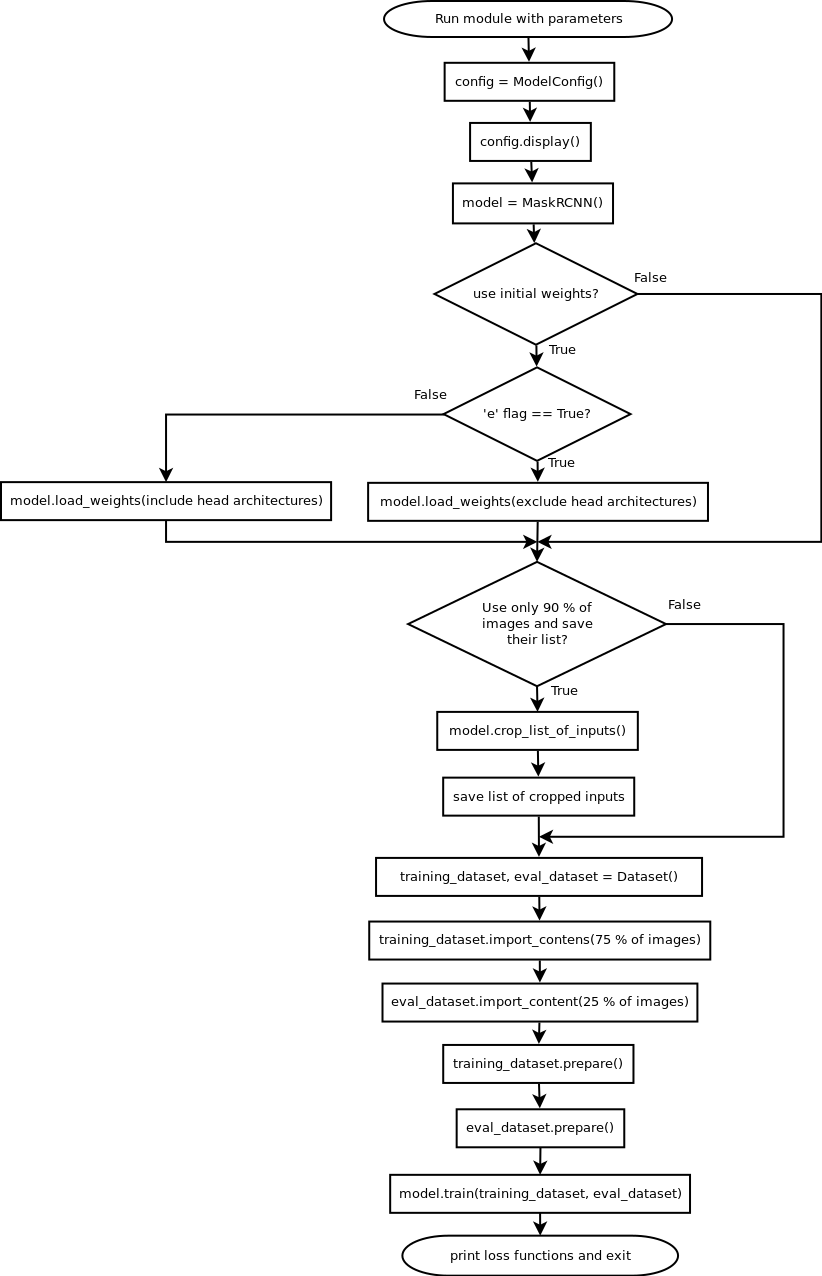
\includegraphics[width=0.95\linewidth]{./pictures/train_dia.png}
	\caption[ann.maskrcnn.train flowchart]{Flowchart of the~ann.maskrcnn.train module}
      \label{fig:train}
\end{figure}

\begin{figure}[H]
   \centering
	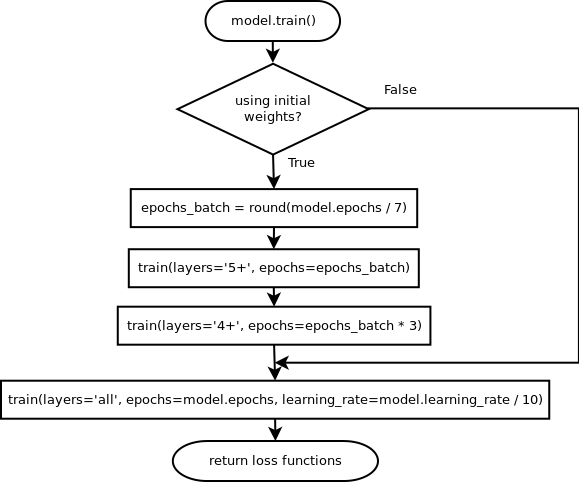
\includegraphics[width=\linewidth]{./pictures/training_dia.png}
	\caption[ann.maskrcnn.train training flowchart]{Flowchart of different training branches inside the~ann.maskrcnn.train module}
      \label{fig:training}
\end{figure}

\verb|ann.maskrcnn.train| also contains its own manual, help and a~graphical 
user interface (\zk{GUI}) to help a~user's understanding of the~module.

\section{ann.maskrcnn.detect}
\label{detect-module}

In case we have a~trained model, either trained by us or provided by someone 
else, we can use it to detect features or objects in maps. Such maps have to be 
raster maps imprted to GRASS GIS or georeferenced raster files. The~output
from the~module consists of a~set of vector 
maps for each class. Although the~model is to some extent scale-invariant, it is 
recommended to provide rasters in similar resolution to the~one used in
training images. The~detection is done in the~\verb|ann.maskrcnn.detect| GRASS GIS
module. The~module is written in the~file \verb|ann.maskrcnn.detect.py| and was 
written for the~practical part of the~thesis. Its workflow is with some 
simplifications illustrated in figure \ref{fig:detect}.

As in the~\verb|ann.maskrcnn.train| module, the~flowchart contains few 
already-mentioned functions and classes, specifically the~\verb|ModelConfig| 
class from chapter \ref{config} and the~\verb|MaskRCNN| class from chapter 
\ref{model-mrcnn}.

However, more unmentioned functions can be seen in the~flowchart. Function
\verb|parse_instances| imports masks of detected instances into GRASS GIS
(except for images with external georeferencing; they are just saved into
a~temporary folder). These masks are rasters of the~same size as the~input
maps/images where mask pixels have the~value of class ID and the~rest are
zeros. In case the~georeferencing is external, a flag \verb|-e| should be
used and the~function \verb|external_georeferencing| is 
called to copy georeferencing files to the~directory with masks and import them
into GRASS GIS.

Rasters are then cropped and vectorized to get a~separate vector map for each
class. The~process of cropping and vectorizing consists of a~bunch of GRASS GIS
modules and is illustrated in figure \ref{fig:vectorize}.

The illustrated process works only with detected classes (e.g. when no instance 
of sties was detected, the~loop corresponding to this class will be skipped). 
The~term \verb|vector_map| used in the~flowchart corresponds to the~same string 
as the~term \verb|raster_map|, but is used to emphasize the~difference in
the~map type; it is also the~reason why we can use \verb|v.patch| and 
\verb|g.remove| with \verb|vector_maps| - because we already have the~list of 
raster maps. The~motivation behind the~inner loop in the~flowchart is
a~detection made on multiple rasters; classes from them are extracted and 
vectorized separately and then patched together for each class.

\begin{figure}[H]
   \centering
	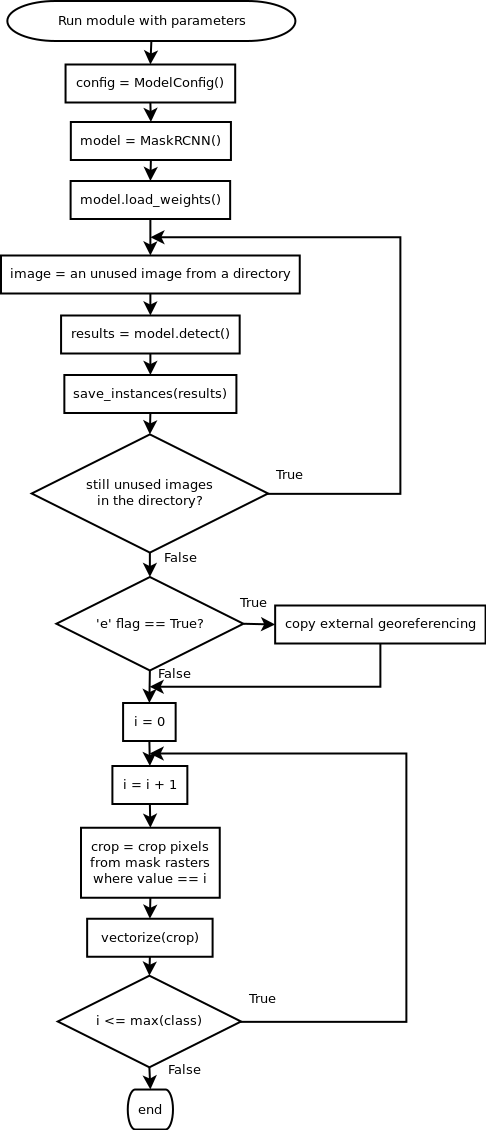
\includegraphics[width=\linewidth]{./pictures/detect_dia.png}
	\caption[ann.maskrcnn.detect flowchart]{Flowchart of the~ann.maskrcnn.detect module}
      \label{fig:detect}
\end{figure}

\begin{figure}[H]
   \centering
	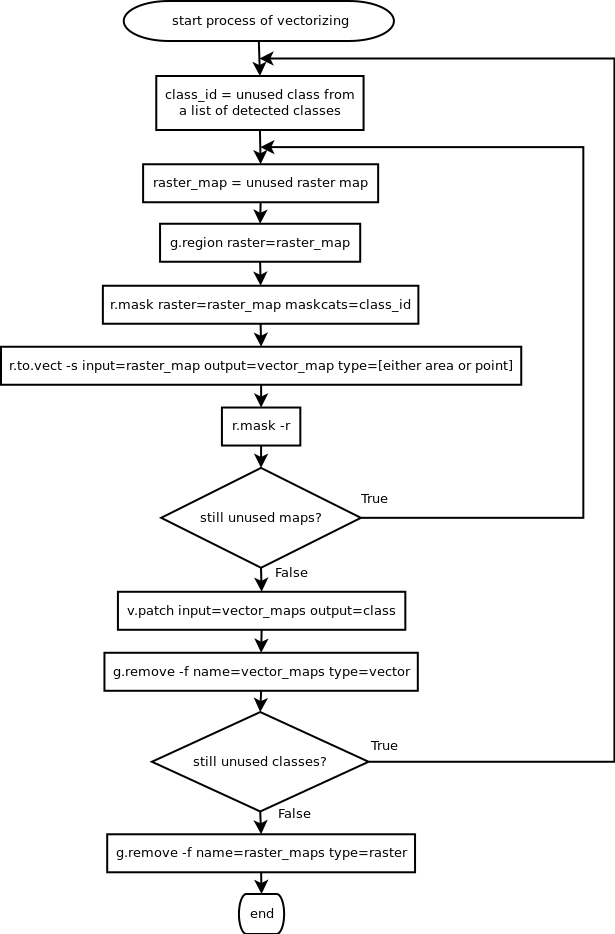
\includegraphics[width=0.95\linewidth]{./pictures/vectorize.png}
	\caption[vectorization in ann.maskrcnn.detect flowchart]{Flowchart of the~vectorization and classes extraction in the~ann.maskrcnn.detect module}
      \label{fig:vectorize}
\end{figure}

The output of \verb|ann.maskrcnn.detect| represents detected masks in a~vector form. The~output type can be either areas or points (corresponding to a~centre of the~mask).

\verb|ann.maskrcnn.detect| also contains its own manual, help and a~\zk{GUI} to 
help a~user's understanding of the~module.

\section{GRASS GIS patch}
\label{grass-patch}

Although the~support for Python 3 in GRASS GIS is a~widely discussed topic and
although much effort has been done to for it, it is still incomplete. This
lack is handled in modules, but there is still a~problem in setting the~GRASS
environment. Thus, a~patch and a~recompilation of GRASS are needed to allow the
user to set the~environment right. The~patch decodes bytes-typed string into a
UTF-8-typed string and consists of the~following \textit{diff}.

{\scriptsize
\begin{lstlisting}[basicstyle={\footnotesize\ttfamily},breaklines=True,
backgroundcolor = \color{light-gray}]
===================================================================
--- lib/python/script/core.py	(revision 72644)
+++ lib/python/script/core.py	(working copy)
@@ -746,7 +746,7 @@
         elif var.startswith(b'opt_'):
             options[var[4:]] = val
         elif var in [b'GRASS_OVERWRITE', b'GRASS_VERBOSE']:
-            os.environ[var] = val
+            os.environ[var.decode("utf-8")] = val.decode("utf-8")
         else:
             raise SyntaxError("invalid output from g.parser: %s" % line)
\end{lstlisting}}
